Assemblando insieme le componeneti derivate dalle entità principali, quindi procedendo da un punto di vista dettagliato ad uno generale, otteniamo il modello ER, seguendo l'approccio misto adottato, in questo caso nella fase BOTTOM-UP.

\begin{landscape} %inizia un foglio landscape

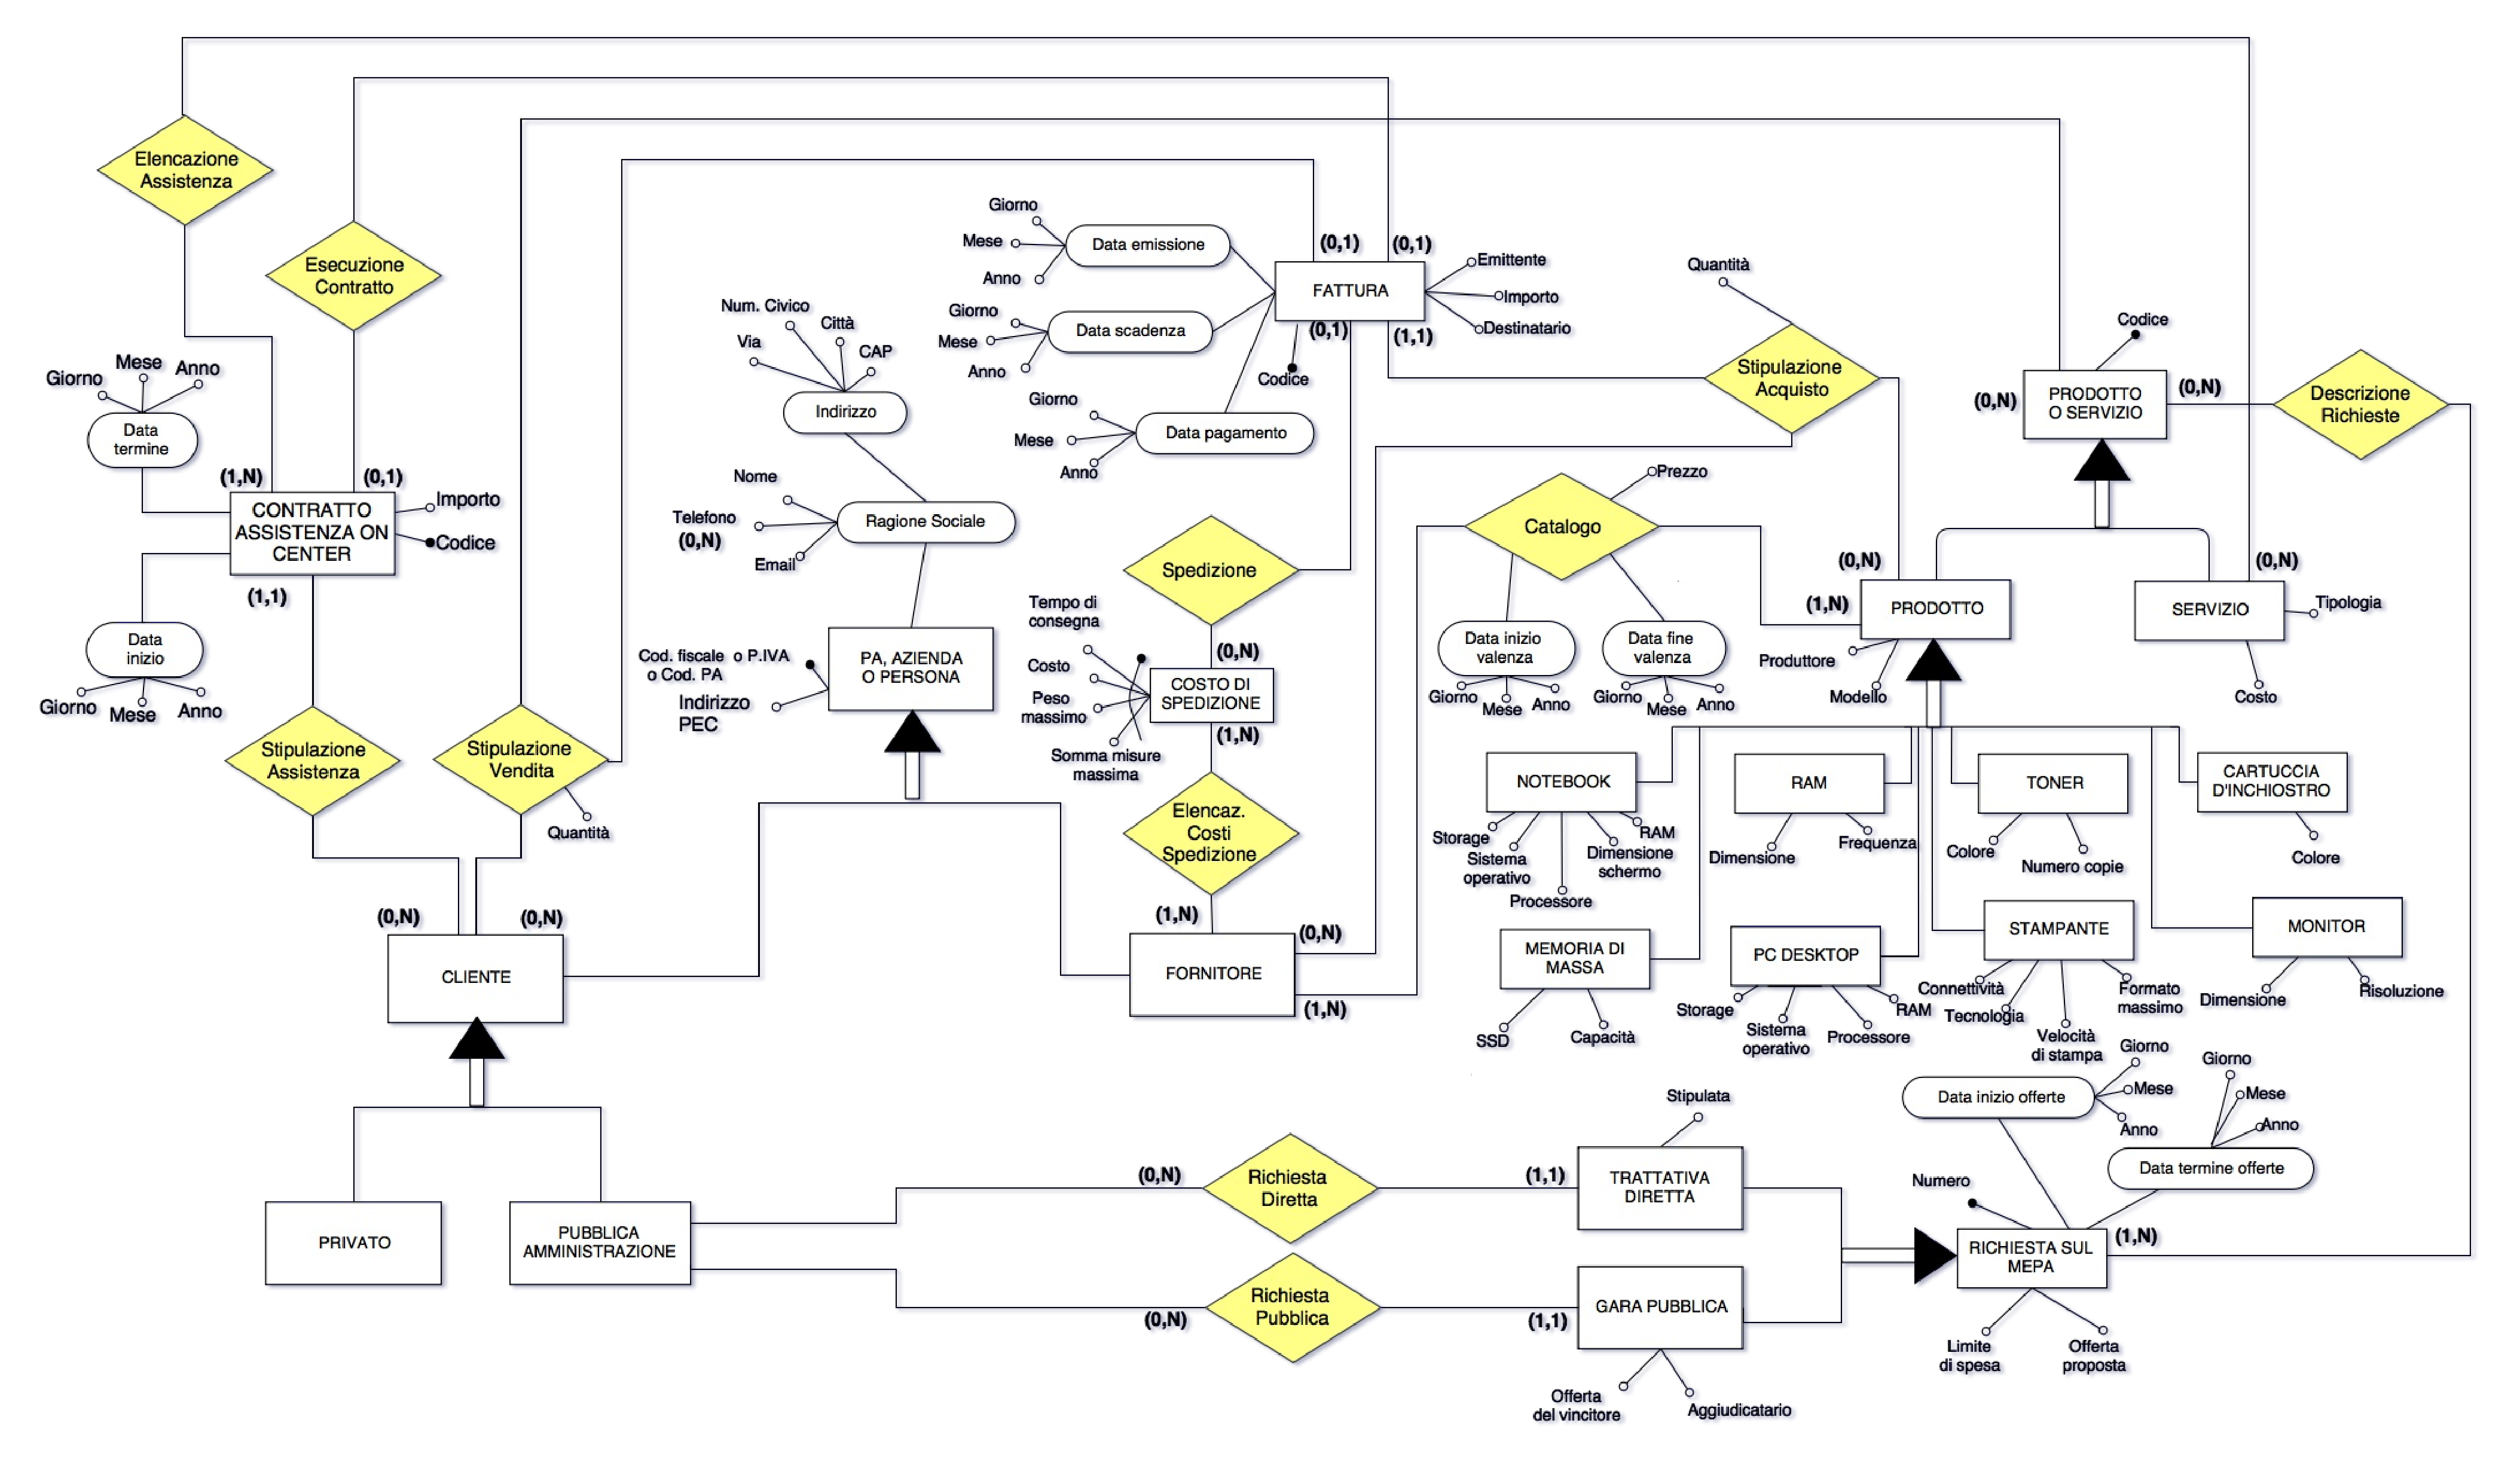
\includepdf[angle=90]{./immagini/modello_er.pdf}

\end{landscape}
% \noindent\makebox[\textwidth]{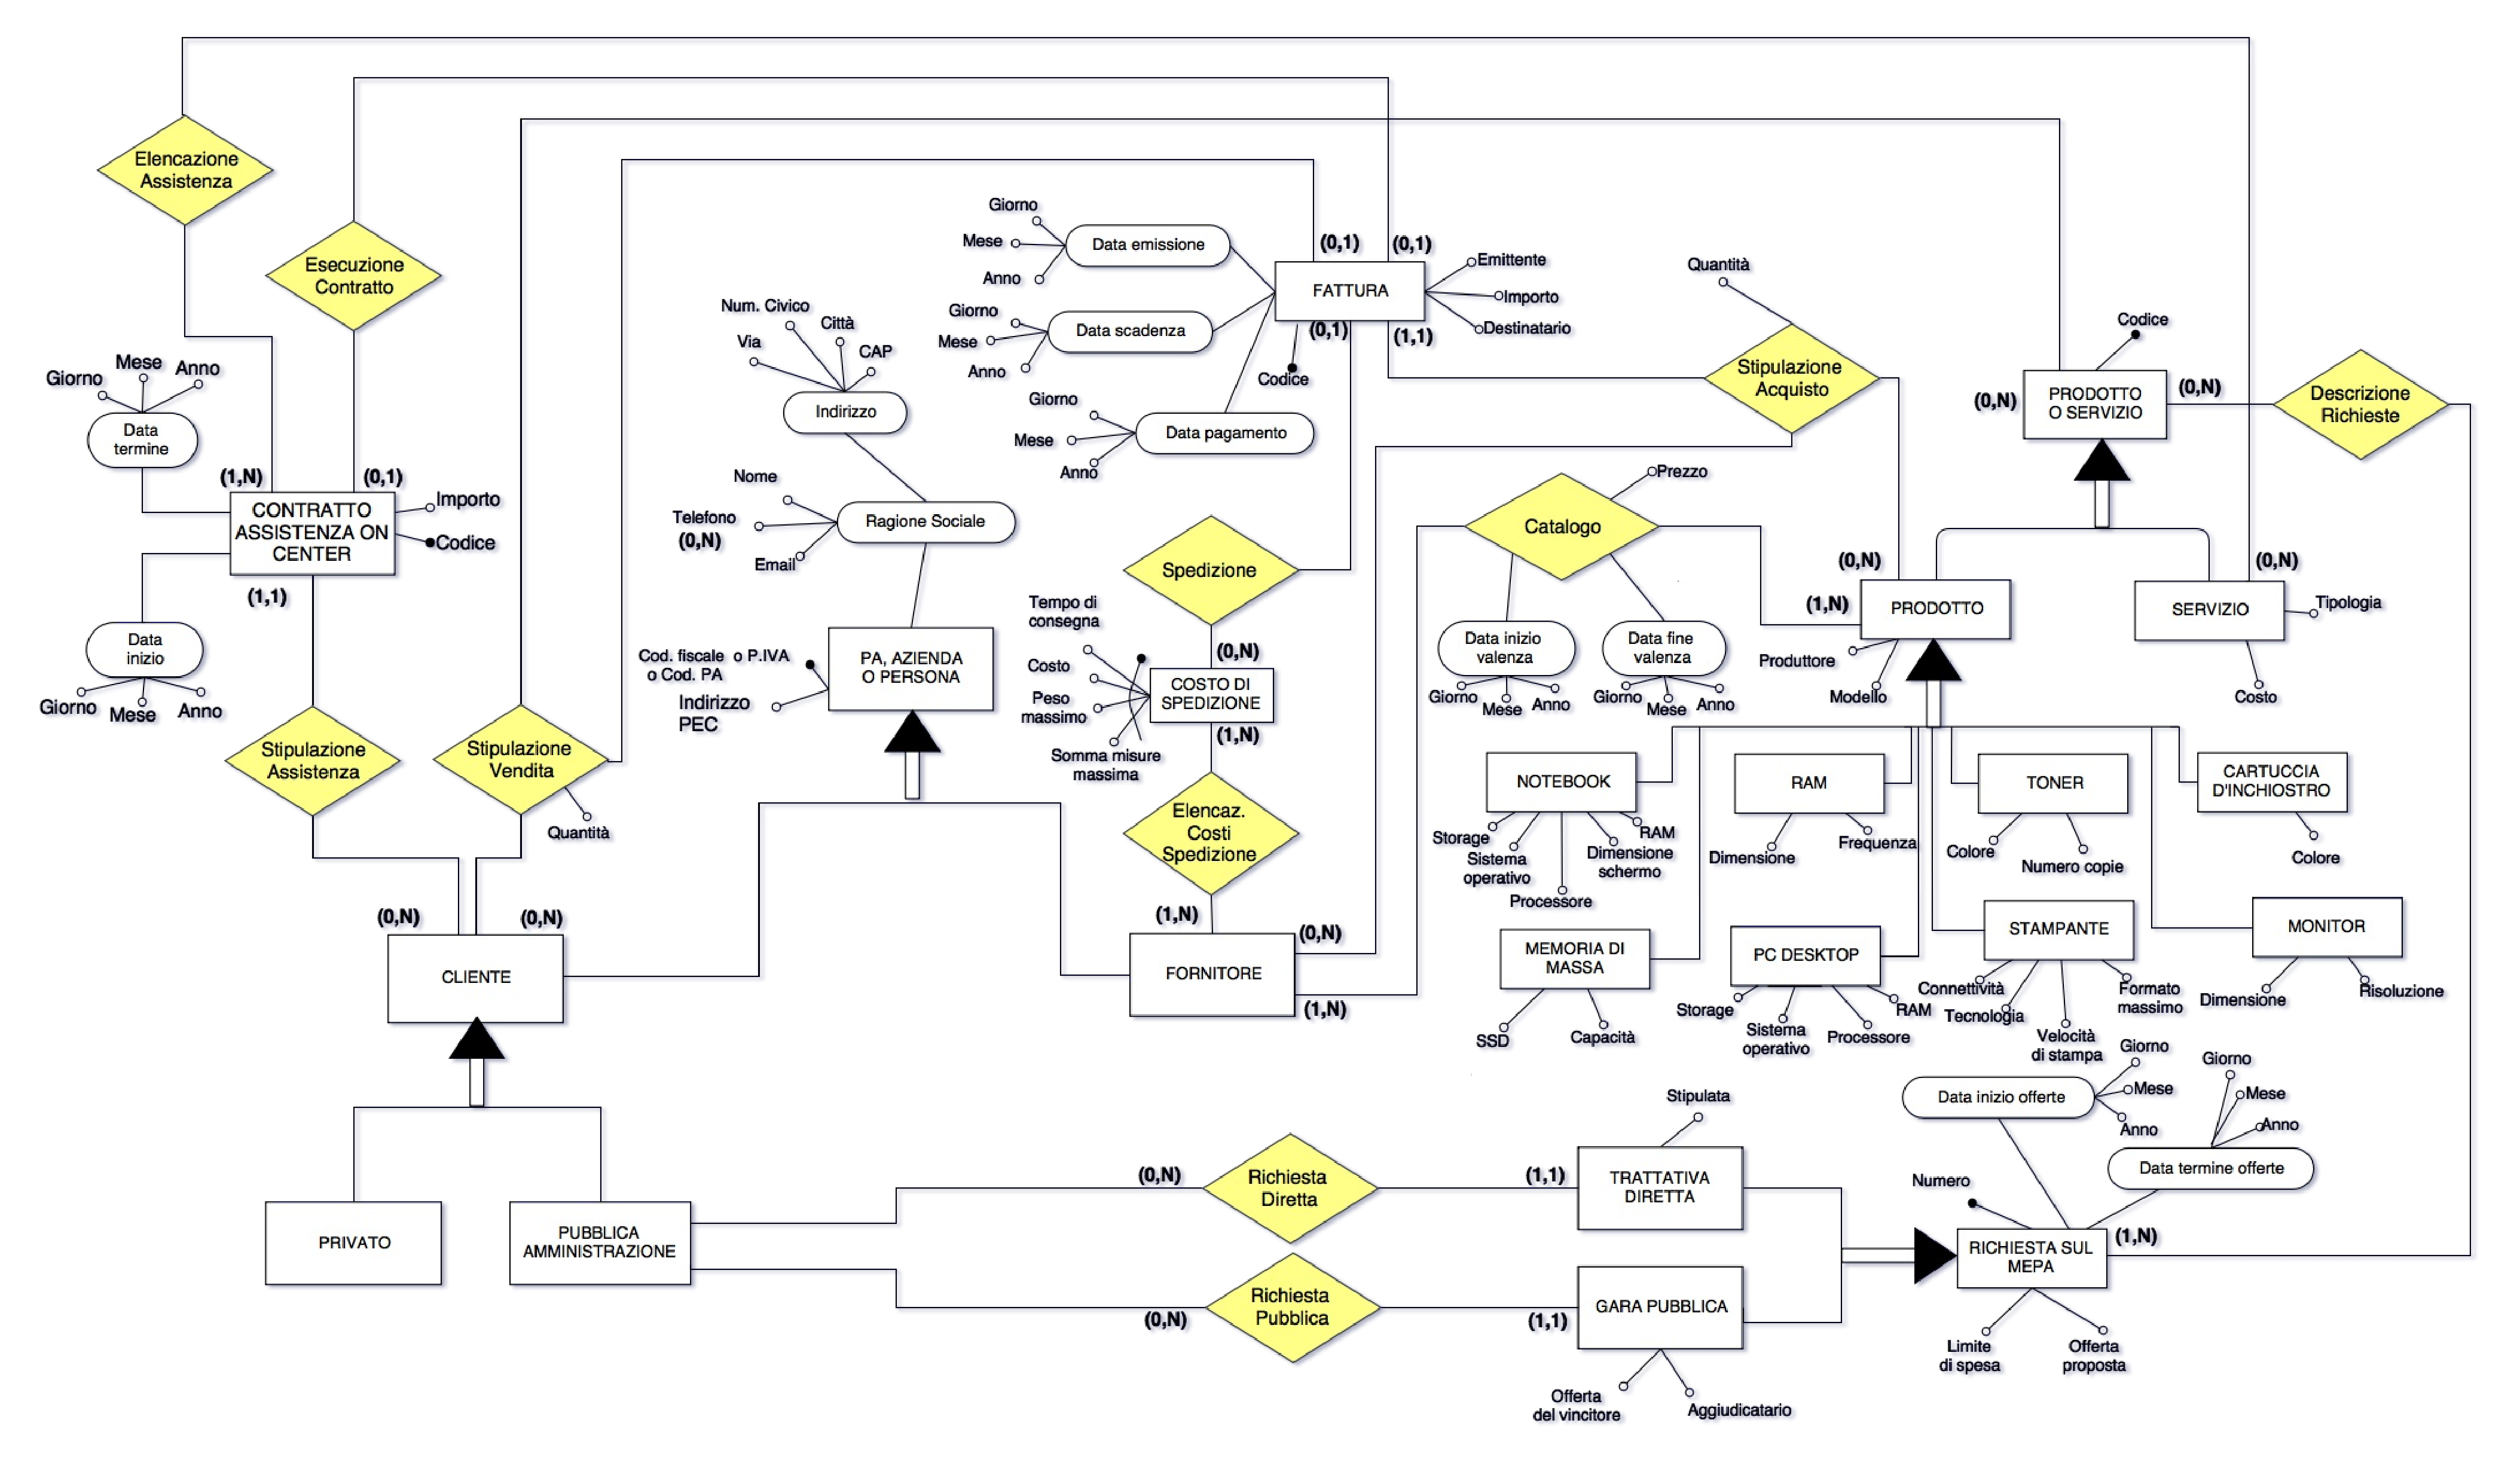
\includegraphics[width=0.9\linewidth]{./immagini/modello_er.pdf}}

Sono state inserite le relationship tra le diverse entità.\newline
Nello specifico si può notare come la Pubblica Amministrazione sia direttamente collegata alla Richiesta sul MEPA, attraverso il tipo di richiesta di offerta a cui l'azienda partecipa, quindi dalle relazioni "Richiesta Pubblica" e "Richiesta Diretta". La stessa richiesta sul MEPA è poi in relazione con Prodotto o Servizio in modo da rappresentare la richiesta sottoposta dalla pubblica amministrazione nella Gara Pubblica o nella Trattativa Diretta con la relazione "Descrizione Richieste".\newline
La Pubblica Amministrazione, in quanto parte del macroblocco dei clienti potrà, come il Privato, ricevere assistenza oppure effettuare un acquisto, ciò si traduce nel primo caso nella relazione "Stipulazione Assistenza" con Contratto di Assistenza On Center, e nel secondo caso nella relazione "Stipulazione di Vendita" con Fattura e Prodotto o Servizio.\newline
A suo volta il Contratto di Assistenza on Center avrà bisogno dei servizi offerti, che derivano dalla relazione "Elencazione Assistenza" proprio con Servizio. In più la stipula del contratto viene siglata con l'emissione di una fattura, infatti qui abbiamo la relazione "Esecuzione Contratto" a testimonianza di questo.\newline
La Fattura viene emessa anche quando l'azienda acquista da un Fornitore. Questa relazione è descritta da "Stipulazione Acquisto", che è anche in relazione con Prodotto, per il prodotto coinvolto nell'acquisto.\newline
Il Fornitore è se stesso in relazione diretta con i Prodotti attraverso la relazione "Catalogo", e con il Costo di Spedizione attraverso la relazione "Elencazione Costi Spedizione", che a sua volta è in relazione con la Fattura con "Spedizione".
\newline
Da questo schema di base si cominciano ad effettuare le analisi per possibili ampliamenti e l'introduzione di ridondanze.
